\section{System Architecture}\label{system-architecture}

\subsection{High-level Architecture}\label{high-level-architecture}

To facilitate a comprehensive understanding of the
system\textquotesingle s architecture, this section presents a
high-level overview of the primary classes and their interactions.
Figure \ref{fig:class_diag1} below provides a simplified visual representation of the class
structure and their relationships. It\textquotesingle s important to
note that this diagram is an abstraction intended to clarify the core
architectural elements; it does not depict every attribute or method
within these classes. The diagram has been constructed using PlantUML
\cite{48}.

\begin{figure}[ht]
  \centering
  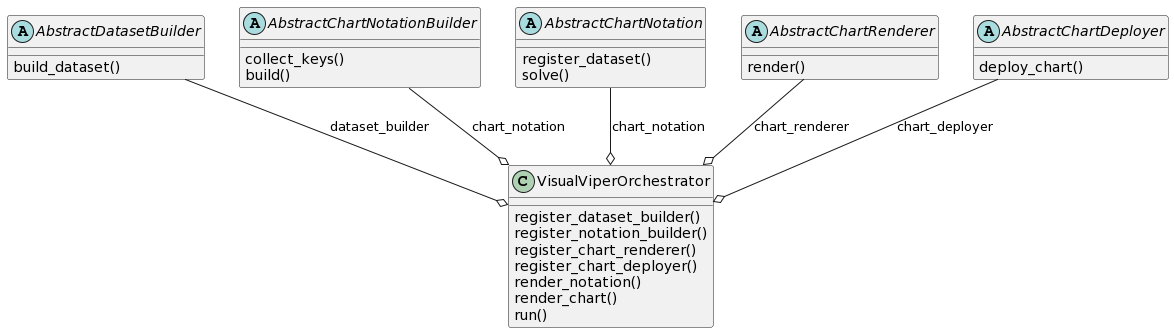
\includegraphics[width=\textwidth]{media/fig8.png}
  \caption{High-level Class Diagram of System Architecture.}
  \label{fig:class_diag1}
\end{figure}

The architecture of the VV system is designed to be both modular and
extensible, adhering to the principles of OOP. This design allows for
high cohesion among components, low coupling between modules, and
promotes scalability. To elaborate on the components that constitute
this architecture, we have categorized them into Abstract Classes,
Concrete Implementations, and an Orchestrator Class.

\subsubsection{Key Classes and
Components}\label{key-classes-and-components}

The Abstract Classes act as templates or interfaces, specifying what
actions must be performed but not how to perform them. Concrete
Implementations are subclasses that provide the specific
\textquotesingle how-to\textquotesingle, the logic and the behavior. The
Orchestrator Class serves as the orchestrating agent that ties these
different components together into a cohesive, functioning system.

\paragraph{Abstract Classes}\label{abstract-classes}

\begin{itemize}
\item
  \textbf{AbstractDatasetBuilder}: Provides the framework for
  constructing datasets.
\item
  \textbf{AbstractChartNotation}: Functions as the foundational class
  for handling chart notations. It provides the methods for registering
  datasets and solving elements.
\item
  \textbf{AbstractChartRenderer}: Serves as the interface for chart
  rendering mechanisms.
\item
  \textbf{AbstractChartDeployer}: Serves as the base class for all chart
  deployment mechanisms.
\end{itemize}

\paragraph{Concrete Implementations}\label{concrete-implementations}

\begin{itemize}
\item
  \textbf{GoogleSpreadsheetDatasetBuilder}: Specially designed to build
  datasets from Google Spreadsheets.
\item
  \textbf{AltairChartRenderer}: A concrete implementation of
  AbstractChartRenderer, which specifically uses Vega-Altair for
  rendering charts \cite{49}.
\item
  \textbf{GdriveChartDeployer} and \textbf{MiroChartDeployer}: These are
  specialized implementations of AbstractChartDeployer designed to
  deploy charts on Google Drive and Miro, respectively.
\end{itemize}

\paragraph{Orchestrator Class}\label{orchestrator-class}

\begin{itemize}
\item
  \textbf{VisualViperOrchestrator}: This class manages the interaction
  between the various components. It references a DatasetBuilder, a
  ChartNotationBuilder, a ChartRenderer, and a ChartDeployer. This
  allows the orchestrator to manage the flow of operations.
\end{itemize}

\subsubsection{Component Interactions}\label{component-interactions}

The VisualViperOrchestrator serves as the fulcrum around which the
entire architecture revolves. It dynamically links to various
components, directing the flow of data and operations throughout the
system. Subclasses of AbstractDatasetBuilder,
AbstractChartNotationBuilder, AbstractChartRenderer, and
AbstractChartDeployer, can be plugged into the orchestrator, thereby
fulfilling the design goals of modularity and extensibility.

\afterpage{%
  \clearpage% To flush out all floats, might not be what you want
  \begin{landscape}
\begin{figure}[ht]
  \centering
  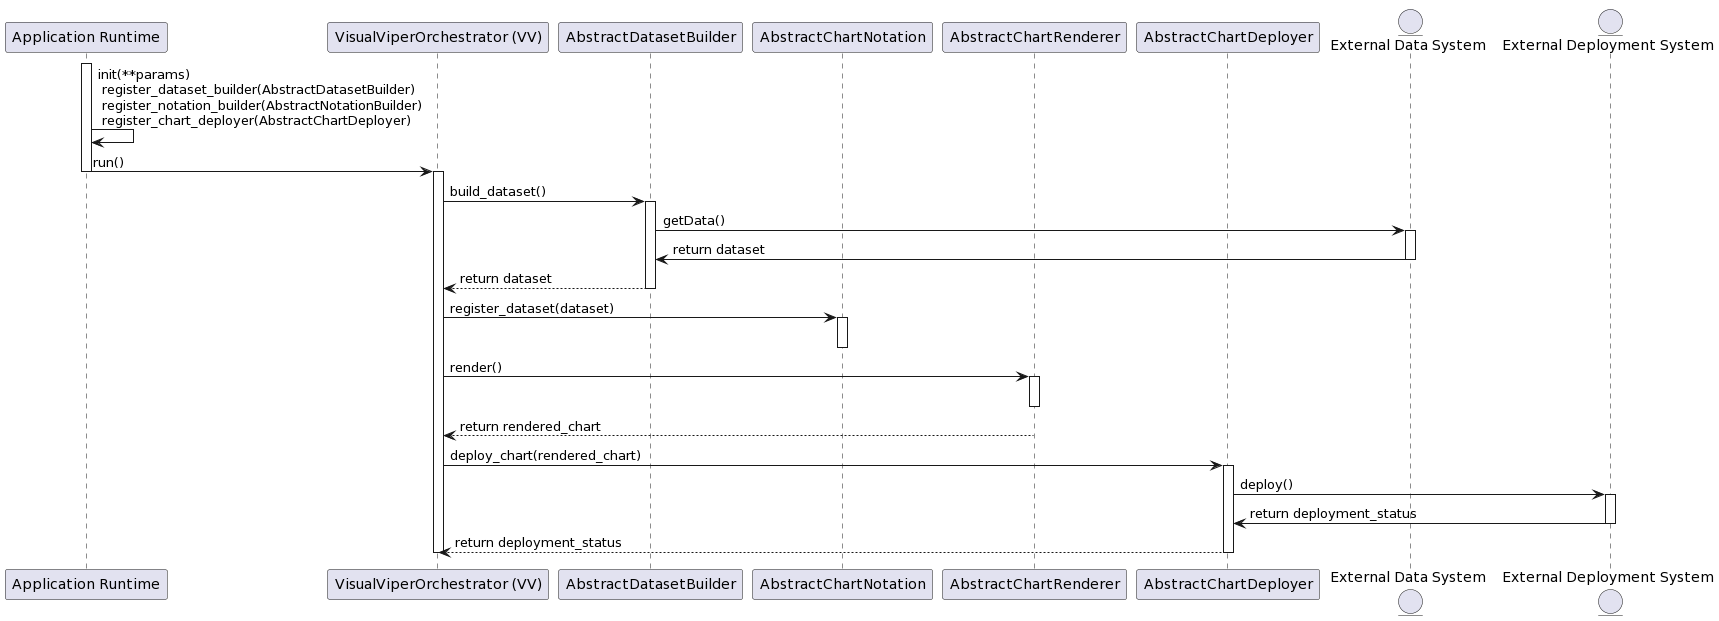
\includegraphics[width=\linewidth]{media/fig9.png}
  \caption{Sequence Diagram for Chart Creation and Deployment in Visual
  Viper Framework.}
  \label{fig:seq_diag}
\end{figure}
\end{landscape}
}

\paragraph{Sequence of Operations}\label{sequence-of-operations}

To provide a more concrete understanding of the interactions between
components, Figure \ref{fig:seq_diag} presents a sequence diagram illustrating the flow
of operations in a typical use case. This diagram was also constructed
using PlantUML.

In this sequence diagram:

\begin{enumerate}
\def\labelenumi{\arabic{enumi}.}
\item
  The Application Runtime initializes the VisualViperOrchestrator and
  registers the required components: AbstractDatasetBuilder,
  AbstractChartNotation, AbstractChartRenderer, and
  AbstractChartDeployer.
\item
  The VisualViperOrchestrator initiates the dataset construction process
  by calling the build\_dataset() method on an AbstractDatasetBuilder
  object. This object may retrieve data from an external system,
  abstracted here for generality.
\item
  Upon successful dataset construction, the VisualViperOrchestrator
  registers the dataset with AbstractChartNotation for further
  processing.
\item
  The VisualViperOrchestrator then invokes the render() method on an
  AbstractChartRenderer object to create the actual visual
  representation.
\item
  Finally, the VisualViperOrchestrator calls the deploy\_chart() method
  on an AbstractChartDeployer object, deploying the rendered chart to an
  external system.
\end{enumerate}

This sequence of operations encapsulates the VV system\textquotesingle s
core functionality while emphasizing its modularity and extensibility.
It serves as an exemplar flow, illustrating how the system components
interact to accomplish the data visualization task.

\subsection{Description of Components}\label{description-of-components}

In this section, we elaborate on the various components of our system,
their roles, and how they interact. To give you a comprehensive
understanding, we\textquotesingle ve included a directory structure in
Figure \ref{fig:folders}.


\begin{figure}[ht]
  \centering
  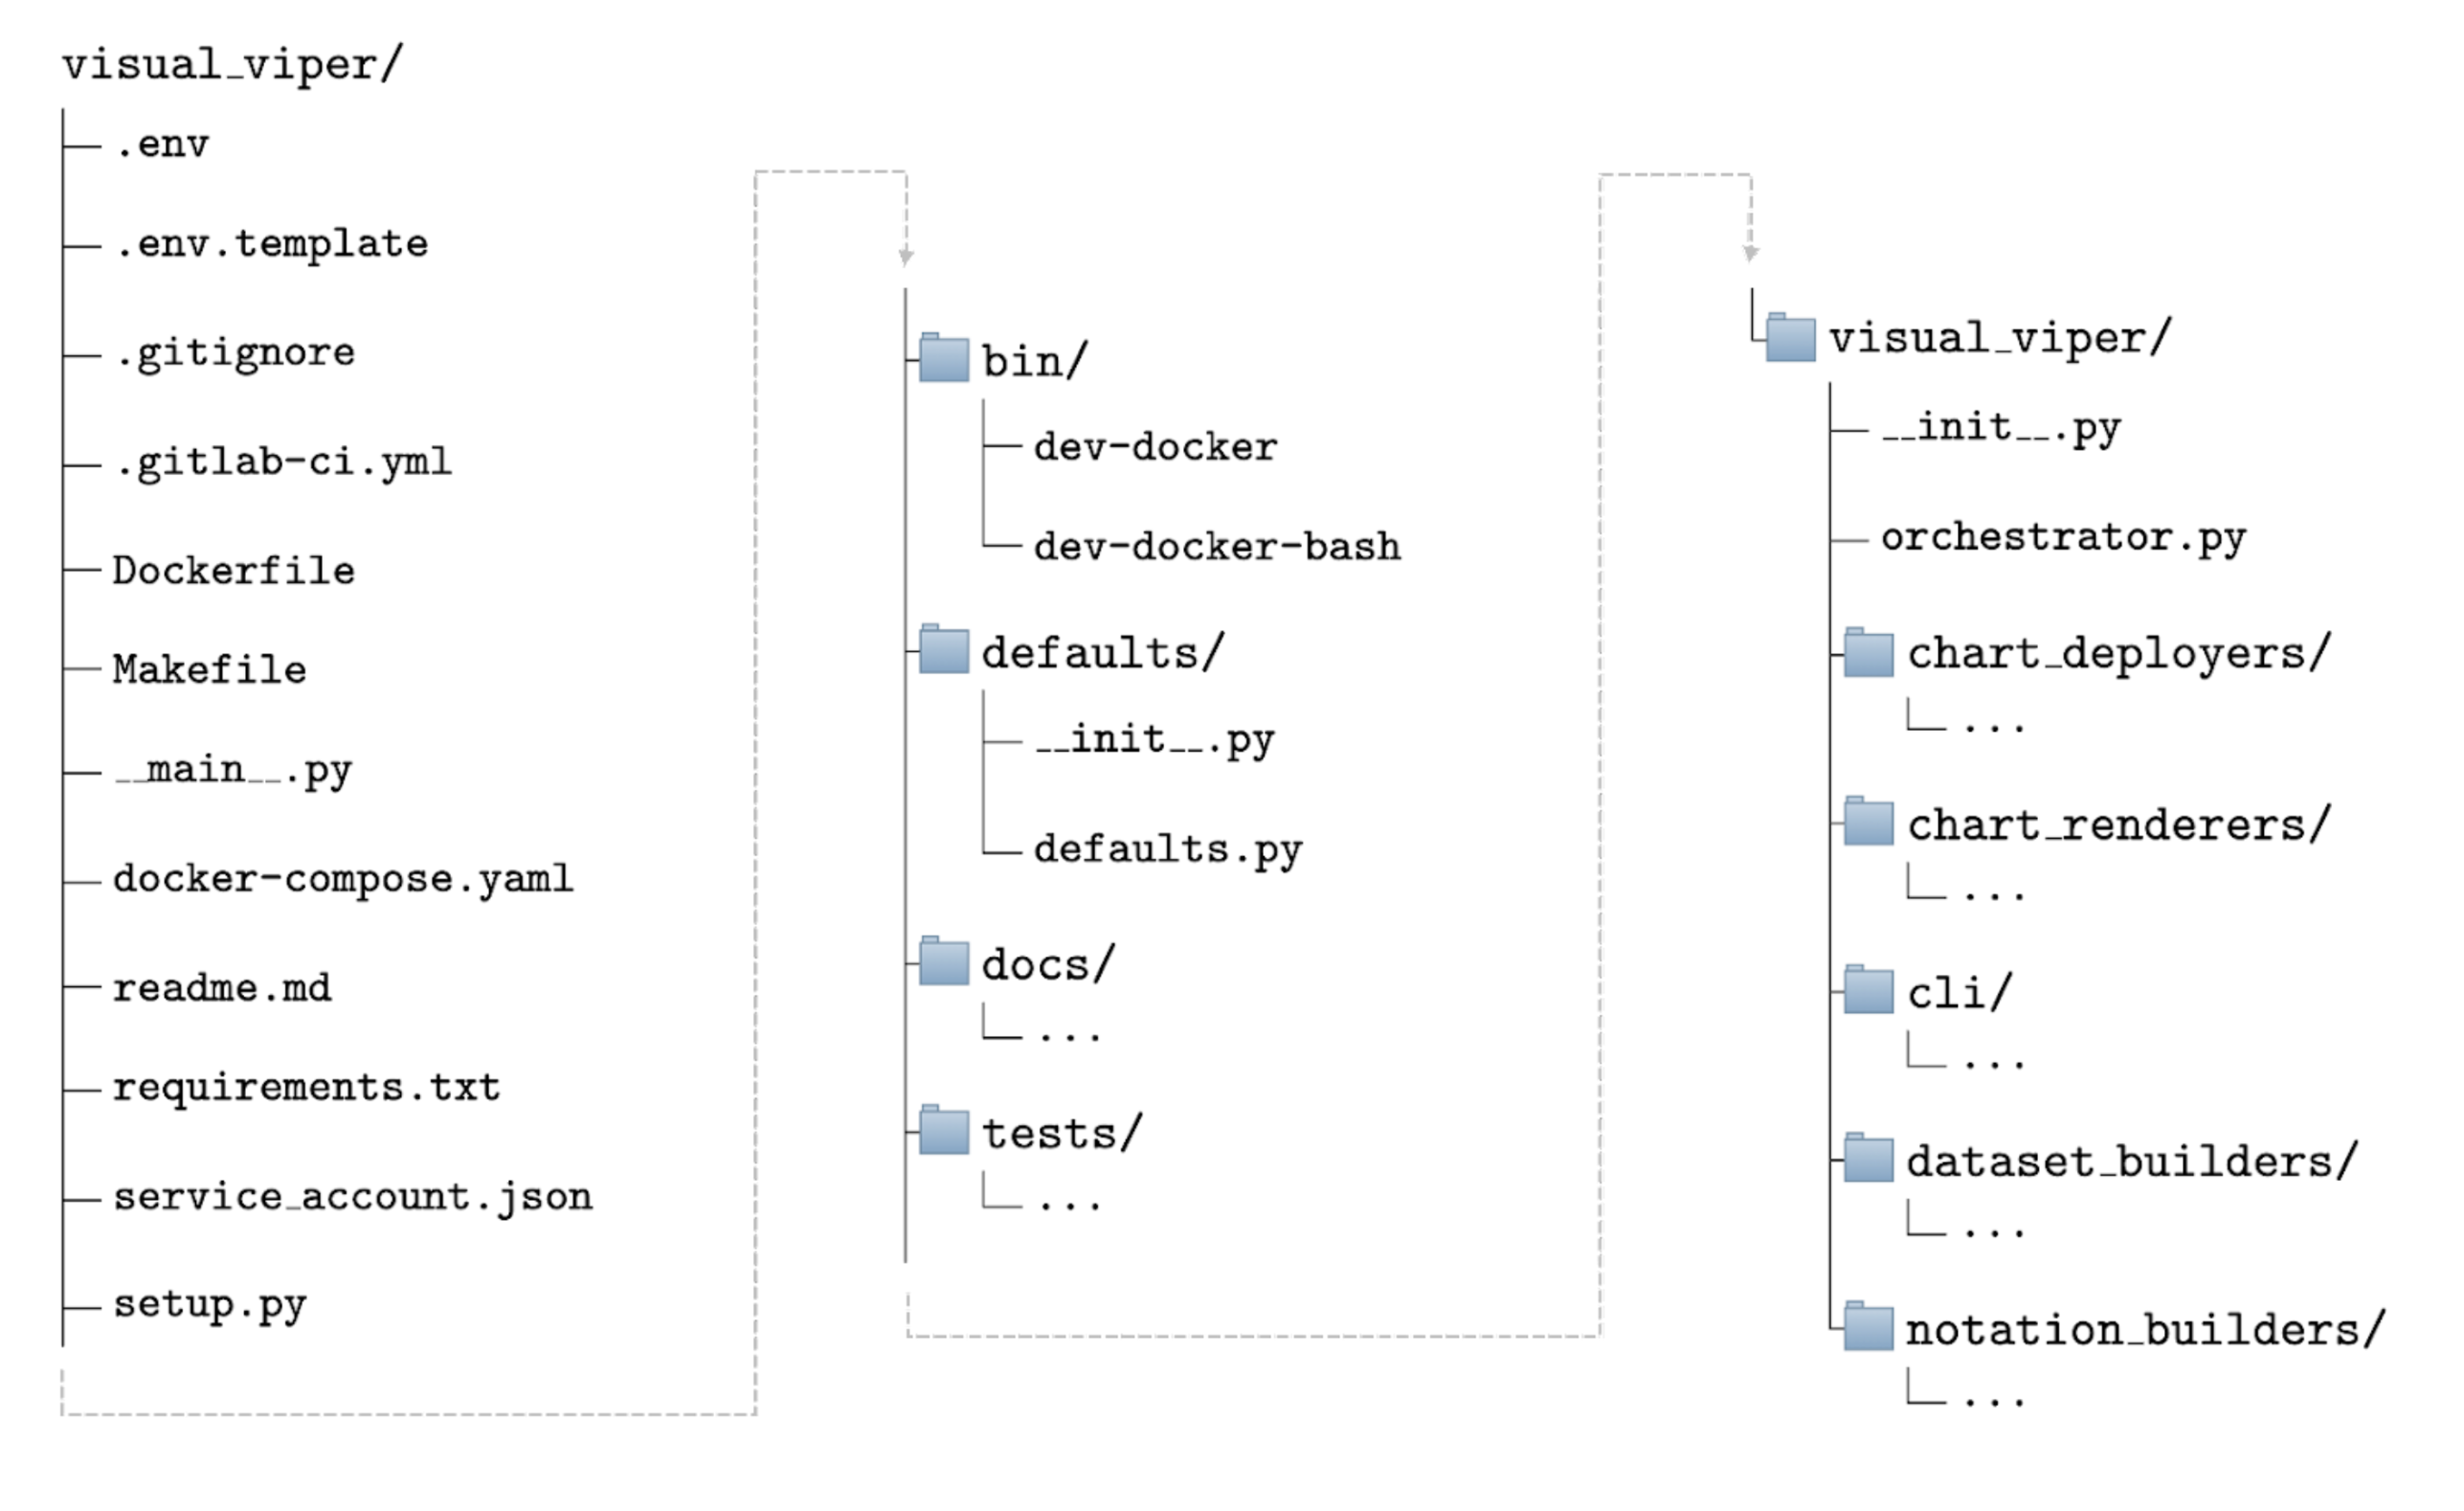
\includegraphics[width=\textwidth]{media/fig10.png}
  \caption{Directory structure of the project. The directory structure
  and the following graphical diagram were generated using
  VV\textquotesingle s directory description and LaTeX diagramming plugins
  (not described in the current work). For brevity, certain folders have
  been excluded or their contents omitted from this diagram.}
  \label{fig:folders}
\end{figure}


\subsubsection{Key Directories and Their Functional
Roles}\label{key-directories-and-their-functional-roles}

\begin{itemize}
\item
  \textbf{defaults/}: This directory contains the default configuration
  settings, enabling the system to operate with a predefined set of
  parameters.
\item
  \textbf{docs/}: Comprising comprehensive documentation, this directory
  aids in the effective utilization and understanding of the system.
\item
  \textbf{tests/}: This is dedicated to unit testing.
\item
  \textbf{visual\_viper/:} This directory encapsulates the core
  functionalities and classes of the project, which include the
  orchestrators and Command-Line Interface (CLI) mechanisms (which is
  still under development).
\end{itemize}

\subsubsection{Alignment with Design
Philosophy}\label{alignment-with-design-philosophy}

The directory structure reflects the project's commitment to modularity
and extensibility, design philosophies that are integral to the project.
The clear demarcation of responsibilities through specialized
directories, such as those for dataset builders, notation builders,
chart renderers, and chart deployers, underscores the project's modular
and extensible architecture.

\subsection{Data Flow among
Components}\label{data-flow-among-components}

To complement the understanding of the system\textquotesingle s
architecture, Figure \ref{fig:data_flow} provides a simplified data flow diagram that
outlines the relationships and interactions among key components. The
diagram was constructed using the DOT language and serves as a
conceptual map for how data is passed and manipulated within the system.

\begin{figure}[ht]
  \centering
  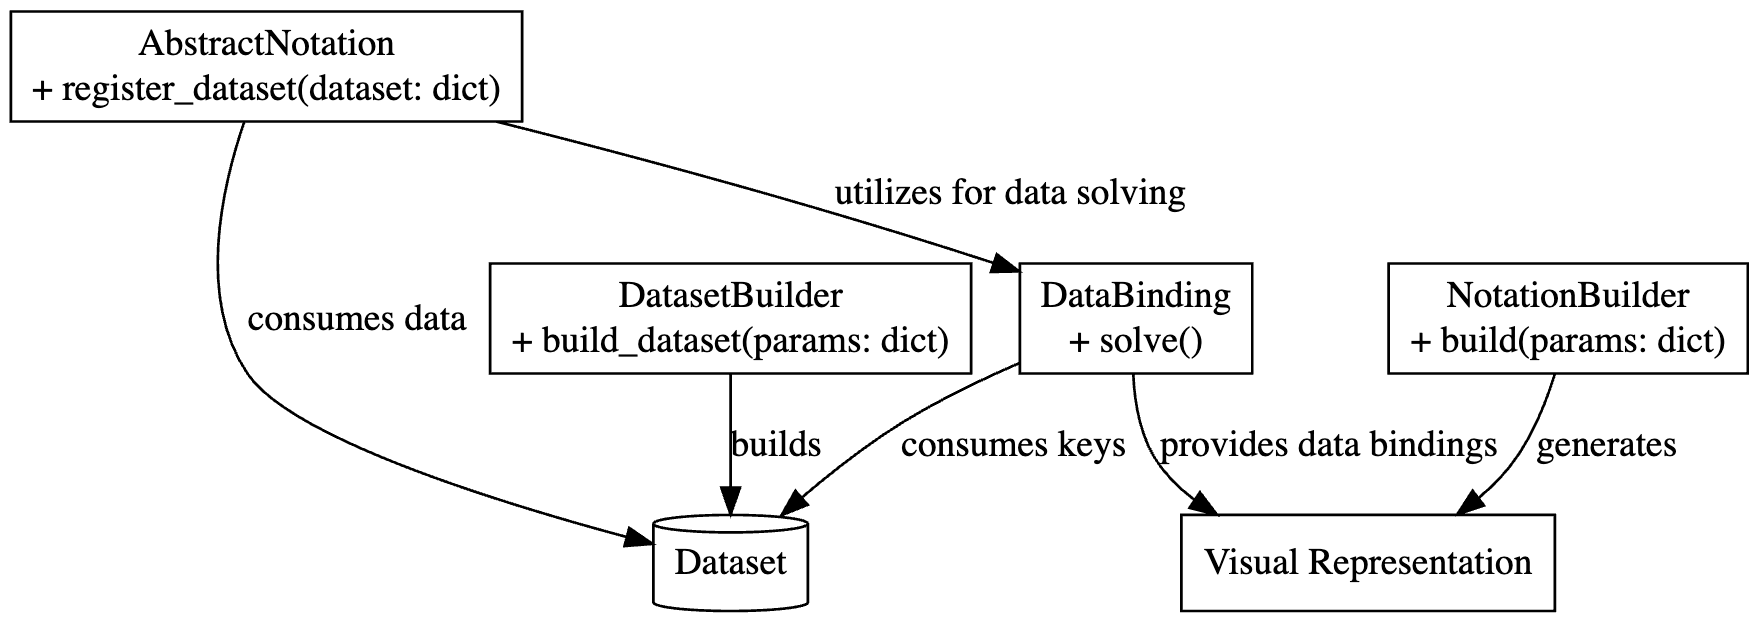
\includegraphics[width=\textwidth]{media/fig11.png}
  \caption{Data Flow Diagram of Key System Components of Visual Viper.}
  \label{fig:data_flow}
\end{figure}

As illustrated in Figure \ref{fig:data_flow}:

\begin{itemize}
\item
  \textbf{DatasetBuilder}: Initiates the process by constructing the
  dataset based on the provided parameters.
\item
  \textbf{Dataset}: Serves as the data store which is consumed by both
  the DataBinding and AbstractNotation classes.
\item
  \textbf{NotationBuilder}: Builds the visual representation of the
  chart, laying out the aesthetics and graphical elements.
\item
  \textbf{Visual Representation}: This is the generated graphical layout
  of the chart, whose appearance is dictated by the NotationBuilder.
\item
  \textbf{DataBinding}: Consumes keys from the Dataset to resolve any
  data dependencies and supplies this resolved data to the visual
  representation.
\item
  \textbf{AbstractNotation}: This class receives data from the Dataset
  and utilizes the DataBinding class to solve for any data-related
  calculations.
\end{itemize}

The DataBinding class plays a crucial role in combining the dataset with
its visual representation, ensuring that the data points are correctly
mapped onto the chart. On the other hand, the AbstractNotation class
establishes the fundamental structure of the chart, including its
underlying logic and computations.

This high-level overview allows for easy plug-and-play of different
dataset builders, data binding mechanisms, and visual representations,
making the system highly modular and extensible.

\subsection{Modular and Extensible Plugin
Architecture}\label{modular-and-extensible-plugin-architecture}

In line with the system\textquotesingle s commitment to modularity and
extensibility, the architecture of VV features a plugin-based mechanism.
This is a crucial subsystem within the broader architecture that enables
users to enhance or alter the functionality without changing the core
codebase. It facilitates a more dynamic, user-driven ecosystem that
aligns with the project\textquotesingle s design philosophy. Below we
describe the key aspects of this plugin architecture.

\subsubsection{Initial Phase Plugins}\label{initial-phase-plugins}

In the initial phase of development, we aimed to build a set of plugins
to meet our most immediate data visualization needs. Specifically, we
focused on the following:

\begin{itemize}
\item
  \textbf{Google Spreadsheet Data Fetcher}: This plugin will serve the
  role of a specialized AbstractDatasetBuilder. It will be designed to
  fetch data from Google Spreadsheets, making it easier for users to
  source data without manual intervention.
\item
  \textbf{Vega-Lite Notation Builders}: A group of specialized
  AbstractChartNotation plugins will be developed to create notations
  for Vega-Lite charts. The focus will initially be on generating Forest
  Plots.
\item
  \textbf{Vega-Altair Chart Renderer}: An implementation of
  AbstractChartRenderer, this plugin will use the Vega-Altair library
  for rendering the visual representation of the charts.
\item
  \textbf{Multi-platform Chart Deployers}: To augment the deployment
  capabilities, we aimed to create two deployer plugins:

  \begin{itemize}
  \item
    \textbf{Google Drive Deployer}: Specialized for storing rendered
    image files in Google Drive, making it convenient for users to
    access and share their visualizations.
  \item
    \textbf{Miro Deployer}: Places the generated charts in Miro boards
    with a predefined layout, aiding in the interpretation and
    comparison of the charts.
  \end{itemize}
\end{itemize}

Our plugin architecture is designed for future expansion, both by our
team and external contributors. It allows for:

\begin{itemize}
\item
  \textbf{User Customization}: Users can tailor the software to their
  needs by adding or removing features.
\item
  \textbf{Easy Maintenance}: Since the core code is not altered when
  adding plugins, system updates are more straightforward.
\item
  \textbf{Community Input}: The architecture is open to contributions
  from others, allowing for further enhancements.
\end{itemize}

This architecture supports the previously described low coupling by
allowing independent development and integration of plugins, and high
cohesion by ensuring each plugin is a self-contained, focused unit of
functionality.
